\documentclass[compress,svgnames]{beamer}
\usepackage[spanish]{babel}
\usepackage[utf8]{inputenc}
\usepackage{graphicx,hyperref,amsmath,amssymb,ragged2e,tabularx,multirow,natbib,bibentry,graphics}
\usepackage{listingsutf8}



	\title{\LaTeX{} Básico}
%\subtitle{Presentación del curso}
\author{Valentín Vergara Hidd}
\institute[UdeC]{Universidad de Concepción}
\date{\today}
%\logo{udec}


\setbeamertemplate{navigation symbols}{}
\usetheme{Madrid}
%\usecolortheme{albatross}
%\usecolortheme[named=Black]{structure}\lstset{% general command to set parameter(s)

\usefonttheme[onlymath]{serif}
\justifying

%\usebackgroundtemplate{\scalebox{0.6}{\includegraphics[width=\paperwidth]{ko.eps}}}
%\pgfdeclareimage[height=1.2cm, width=1cm]{logo}{udec}
%\logo{\pgfuseimage{logo}}

\begin{document}
\lstset{% general command to set parameter(s)
	language=[LaTeX]TeX,
	basicstyle=\scriptsize\ttfamily, % print whole listing small
	keywordstyle=\color{cyan},
	framexleftmargin=-2pt,
	backgroundcolor=\color{gray!10},
	frame=single,
	tabsize=2,
	rulecolor=\color{black!30},
	title=\lstname,
	escapeinside={\%*}{*)},
	breaklines=true,
	breakatwhitespace=true,
	framextopmargin=-5pt,
	framexbottommargin=-5pt,
	extendedchars=false,
	inputencoding=utf8,
	literate={á}{{\'{a}}}1, 
	literate={é}{{\'{e}}}1,	
	literate={ó}{{\'{o}}}1,
	literate={ú}{{\'{u}}}1,
	literate={ñ}{{\~{n}}}1, 
	literate={í}{{\'{i}}}1
}

%\renewcommand{\listtablename}{Índice de tablas} 
%\renewcommand{\tablename}{Tabla} 

\begin{frame}
\titlepage
\end{frame}

\begin{frame}
\justifying
Esta obra está publicada bajo una Atribución-No Comercial-Licenciar Igual 2.0 Chile de Creative Commons. Para ver una copia de esta licencia, visite

\url{http://creativecommons.org/licenses/by-nc-sa/2.0/cl/.}
\begin{figure}[b]
\centering
\scalebox{0.8}{
\includegraphics{cero}}
\end{figure}
\end{frame}

\begin{frame}{Funcionamiento de \LaTeX{}}{Extremadamente simplificado}
\begin{figure}[H]
	\centering
\scalebox{0.18}{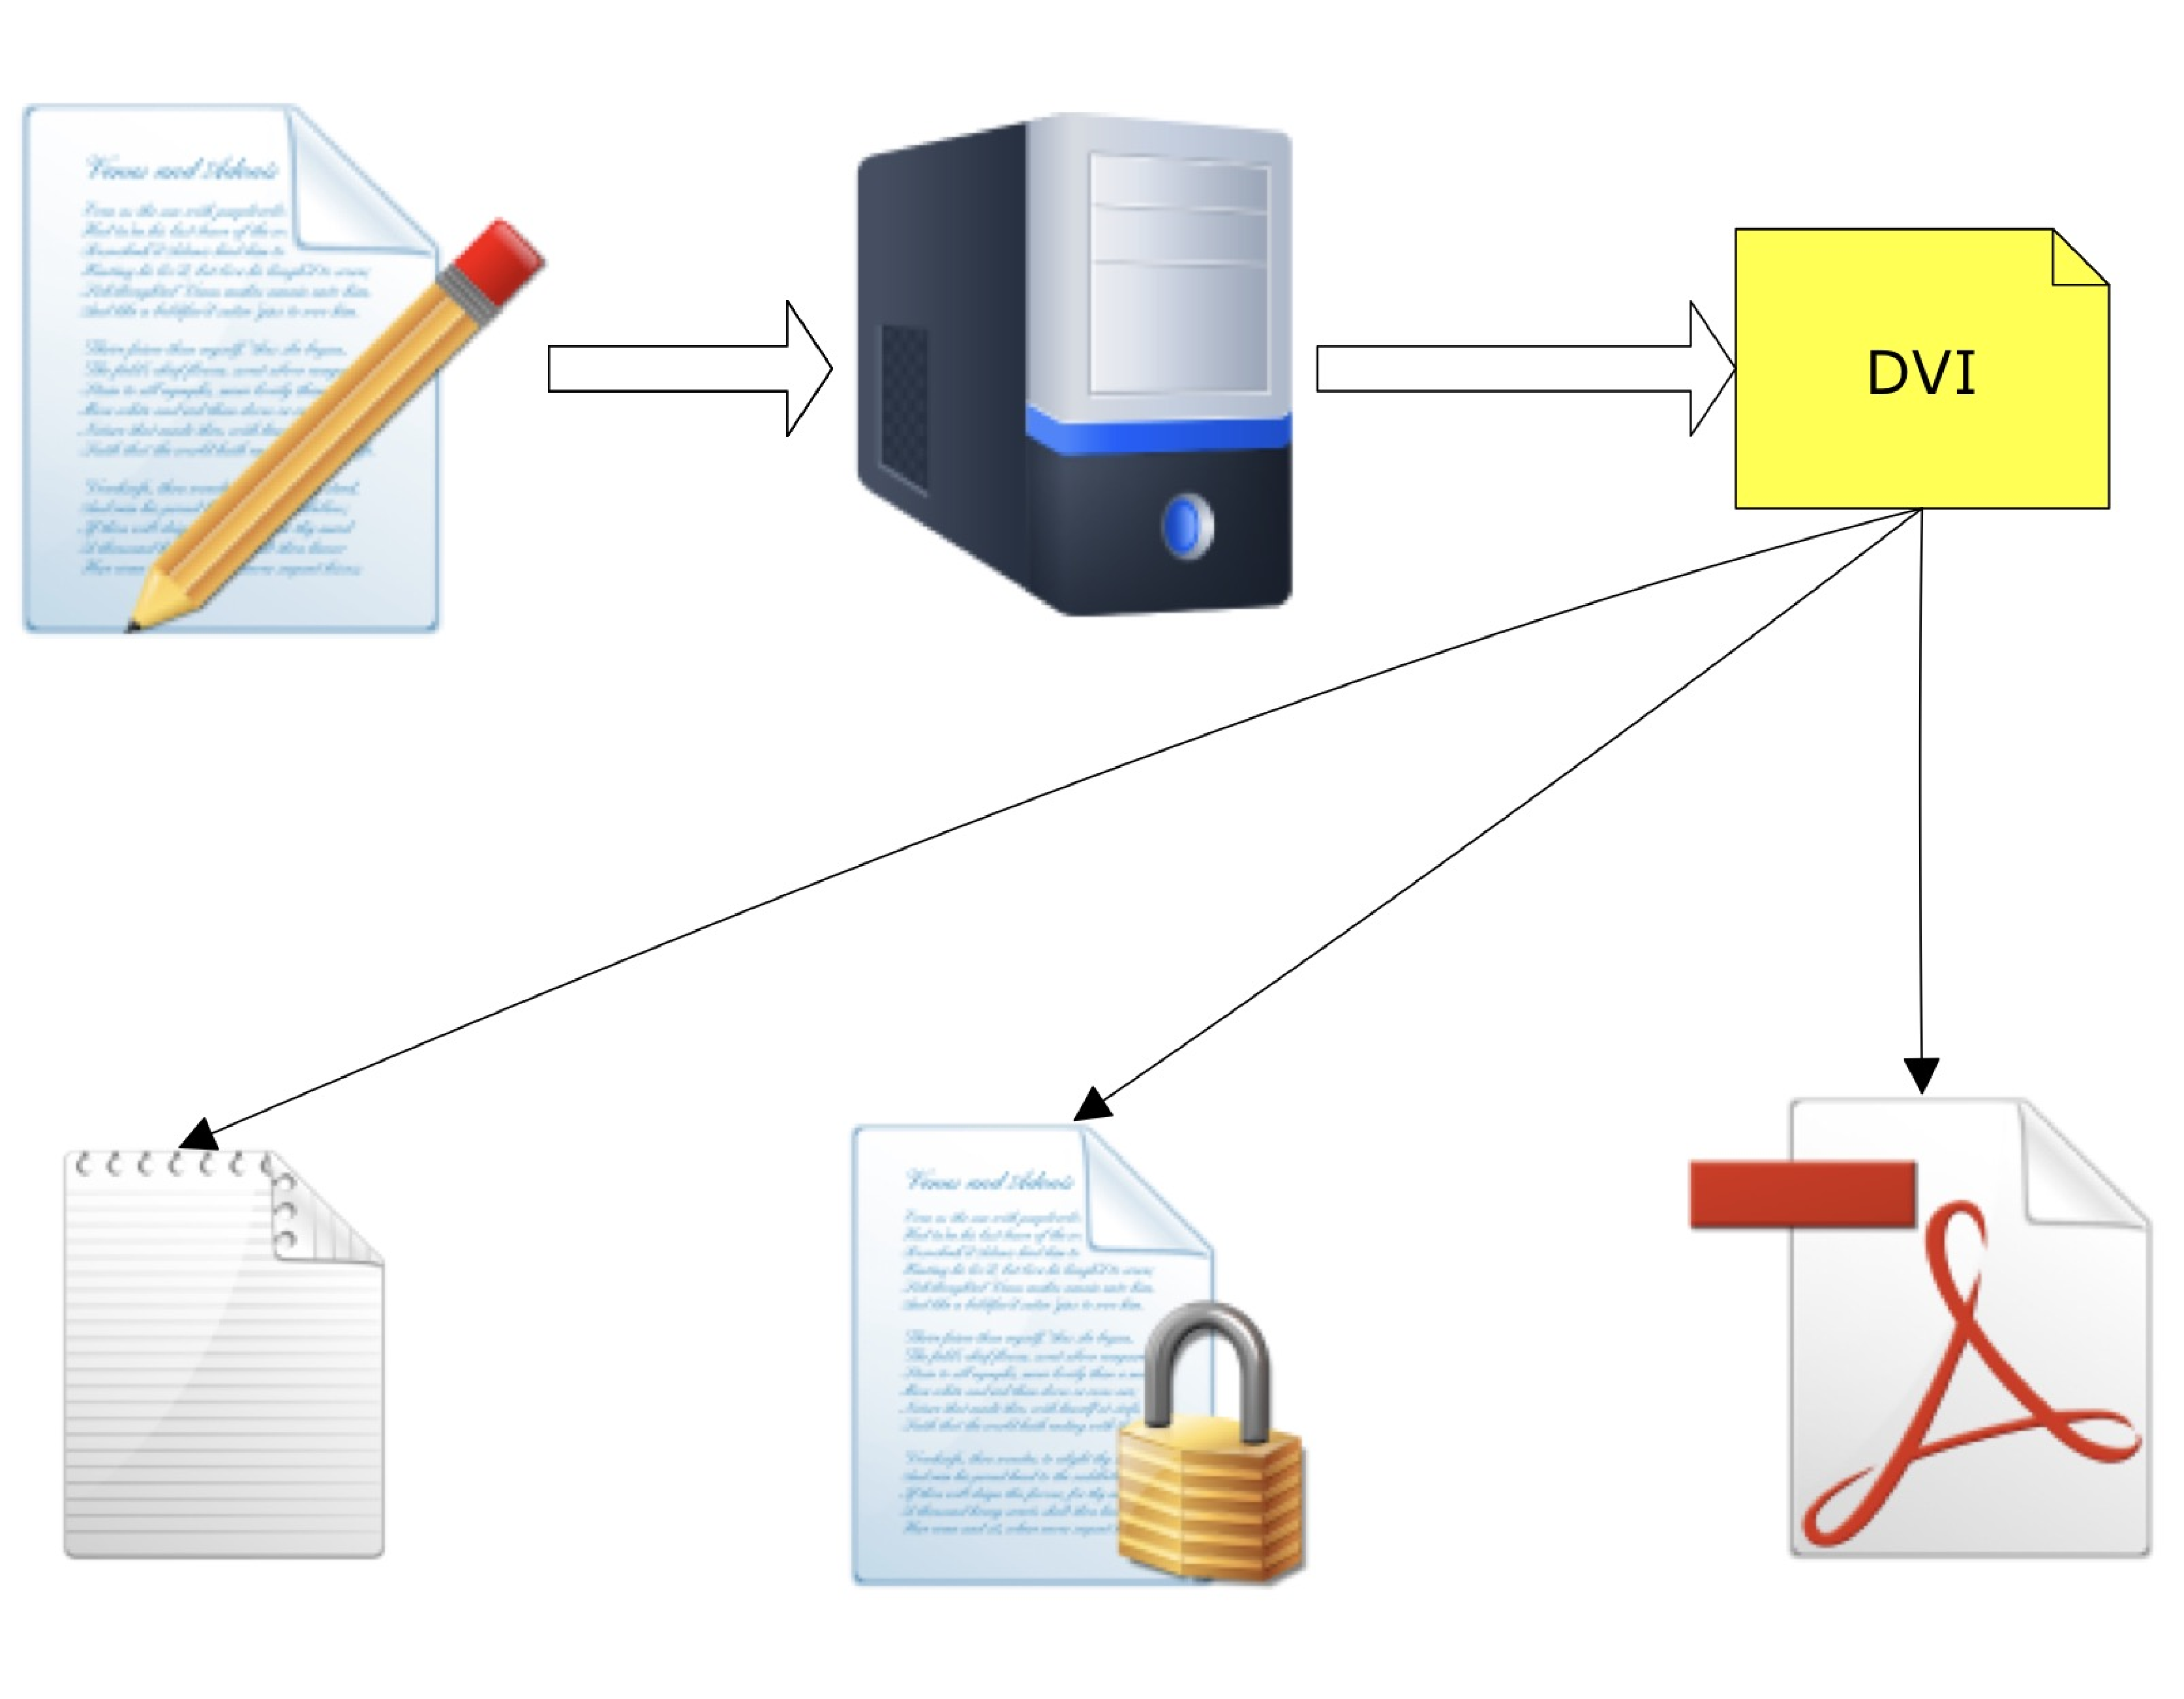
\includegraphics{01_01}}
\end{figure}
\end{frame}

%Listings package

\begin{frame}[fragile]{Para comenzar}
Los documentos en \LaTeX{} comienzan un con {\bf preámbulo}, donde indican opciones globales e instalación de paquetes relevantes. Un preámbulo de documento se debería ver más o menos así
\begin{lstlisting}
\documentclass[letterpaper]{article}

\usepackage[spanish]{babel}
\usepackage[utf8]{inputenc}
\usepackage{amssymb,amsmath,hyperref,graphicx,ragged2e,float}

\author{Valentín Vergara Hidd}
\title{Título del documento}
\date{\today}
\end{lstlisting}

Se pueden ver tres \emph{partes} del preámbulo: Clase global, carga de paquetes e identificación del documento.
\end{frame}


\begin{frame}[fragile]{Entornos}
Como ya se habrán dado cuenta, las \emph{instrucciones}\footnote{Se pueden pensar en estas instrucciones como funciones} que usa R comienzan con un \emph{backslash}. Además, existen ciertos entornos, a los que se accede de la misma forma:
\begin{lstlisting}
\begin{nombre del entorno}
CONTENIDO
\end{nombre del entorno}
\end{lstlisting}

Esto se ocupa principalmente con los siguientes argumentos:
\begin{itemize}
	\item document (¡el más importante!)
	\item itemize
	\item enumerate
	\item equation
	\item Entre otros
\end{itemize}
\end{frame}

\begin{frame}[fragile]{Estructura de los documentos}
Generalmente, los documentos más básicos de \LaTeX{} (article) utilizan una estructura anidada. Es decir, se divide el texto en secciones, que a su vez se dividen en subsecciones, que por su parte también se dividen.\\
El esquema, con su código es como sigue.

\begin{itemize}
	\item Las secciones se crean con el siguiente código:
	\begin{lstlisting}
	\section{Título de la sección.}
	\end{lstlisting}
	\item La división de las secciones:
	\begin{lstlisting}
	\subsection{Título.}
	\end{lstlisting}
	\item La división de las subsecciones:
	\begin{lstlisting}
	\subsubsection{Título.}
	\end{lstlisting}
\end{itemize}
\end{frame}

\begin{frame}[fragile]{Viñetas y listas numeradas}
Para viñetas:
\begin{columns}
	\begin{column}{0.5\textwidth}
		\begin{itemize}
			\item Primer item
			\item Segundo item
			\item (\ldots)
			\item Enésimo item
		\end{itemize}
	\end{column}
	\begin{column}{0.5\textwidth}  
\begin{lstlisting}
	\begin{itemize}
		\item Primer item
		\item Segundo item
		\item (\ldots)
		\item Enésimo item
	\end{itemize}
\end{lstlisting}
	\end{column}
\end{columns}
Para listas numeradas:
\begin{columns}
	\begin{column}{0.5\textwidth}
		\begin{itemize}
			\item Primer item
			\item Segundo item
			\item Tercer item
		\end{itemize}
	\end{column}
	\begin{column}{0.5\textwidth} 
	\begin{lstlisting}
		\begin{itemize}
			\item Primer item
			\item Segundo item
			\item Tercer item
		\end{itemize}
	\end{lstlisting}
	\end{column}
\end{columns}
\end{frame}

\begin{frame}[fragile]{Instrucciones para formateo de texto}
Existen muchas otras, pero las que más se usan son:
\begin{itemize}
	\item {\bf Para texto en negrita}
	\begin{lstlisting}
	{\bf Texto}
	\end{lstlisting}
	\item \emph{El texto en cursiva}
	\begin{lstlisting}
	\emph{Texto}
	\end{lstlisting}
	\item \underline{Para subrayar (no recomendado)}
	\begin{lstlisting}
	\underline{Texto}
	\end{lstlisting}
\end{itemize}
\end{frame}

\begin{frame}[fragile]{Instrucciones para formateo de texto}
	Como se mencionó anteriormente, las instrucciones de \LaTeX{} se pueden tratar como funciones, por lo que es posible combinarlas. Así, el siguiente código:
	\begin{lstlisting}
	\underline{\emph{{\bf Texto en negrita y subrayado}}}
	\end{lstlisting} 
	Produce {\bf \underline{Texto en negrita y subrayado}}	
\end{frame}

\begin{frame}[fragile]{Editor de ecuaciones}
Una de las principales utilidades que se le da a \LaTeX{} es la posibilidad de escribir ecuaciones ---y en general--- lenguaje matemático de forma profesional. Por ejemplo, uno de los usos más comunes que le daremos es la representación de un modelo de regresión multivariada.
\begin{equation}
y = \beta_{0} + \beta_{1}x_{1} + \beta_{2}x_{2} + \beta_{3}x_{3} + \ldots + \beta_{k}x_{k} + \epsilon 
\end{equation}
que se produce con el siguiente código:
\begin{lstlisting}
\begin{equation}
y = \beta_{0} + \beta_{1}x_{1} + \beta_{2}x_{2} + 
\beta_{3}x_{3} + \ldots + \beta_{k}x_{k} + \epsilon 
\end{equation}
\end{lstlisting}
\end{frame}

\begin{frame}[fragile]{Editor de ecuaciones}
Se pueden escribir expresiones con distinto grado de complejidad, como por ejemplo la función de distribución normal acumulada:
\begin{equation}
\phi (x) = \frac{1}{\sqrt{2 \pi}} \int_{-\infty}^{x}e^{-\frac{y^{2}}{2}}dy
\end{equation}
que se produce con el siguiente código:
\begin{lstlisting}
\begin{equation}
\phi (x) = \frac{1}{\sqrt{2 \pi}} 
\int_{-\infty}^{x}e^{-\frac{y^{2}}{2}}dy
\end{equation}
\end{lstlisting}
\end{frame}

\begin{frame}[fragile]{Editor de Ecuaciones}
Se puede optar por no enumerar las ecuaciones, si queremos escribir algo que no guarda relación con las ecuaciones \emph{principales}. Por ejemplo, si nos interesa escribir la identidad de Euler (un ejemplo de belleza matemática), el código es:
\begin{lstlisting}
\begin{equation*}
e^{i \pi} + 1 = 0
\end{equation*}
\end{lstlisting}
lo que produce
\begin{equation*}
e^{i \pi} + 1 = 0
\end{equation*}
\end{frame}

\begin{frame}[fragile]{Editor de Ecuaciones}
	También podemos optar por escribir las ecuaciones en el texto. Por ejemplo:
	\begin{lstlisting}
	``Podemos aprovechar una característica de los logaritmos, 
	tal que $\log ab = \log a + \log b$ ...''
	\end{lstlisting}
	Para producir:\\ ``Podemos aprovechar una característica de los logaritmos, tal que 
	$\log ab = \log a + \log b$ ...''
\end{frame}

\begin{frame}[fragile]{Tablas}
De forma muy frecuente resumimos información en Tablas, que en \LaTeX{} se producen de forma profesional y sin preocupación excesiva por el formato. Por ejemplo:
\begin{table}[H]
\centering
\caption{Aquí se puede poner un título a la Tabla}
\begin{tabular}{lcrr}
\hline \hline 
Columna 1				& Columna 2				& Columna 3				& Columna 4\\
\hline 
Texto					& $f(x) = x^{2}$		& 0.67					& -6.45\\
Más texto				& Texto centrado		& 3.16					& -1.15\\
\hline \hline
\end{tabular}
\end{table}
\end{frame}

\begin{frame}[fragile]{Tablas}
La Tabla Anterior se produce con el siguiente código:
\begin{lstlisting}
	\begin{table}[H]
	\centering
	\caption{Aqui se puede poner un titulo a la Tabla}
	\begin{tabular}{lcrr}
	\hline \hline 
	Columna 1				& Columna 2				& Columna 3				& Columna 4\\
	\hline 
	Texto					& $f(x) = x^{2}$		& 0.67					& -6.45\\
	Mas texto				& Texto centrado		& 3.16					& -1.15\\
	\hline \hline
	\end{tabular}
	\end{table}
\end{lstlisting}
\end{frame}

\begin{frame}[fragile]{Tabla $\neq$ Cuadro}
Por defecto, \LaTeX{} agrega la palabra \emph{cuadro} en lugar de \emph{tabla}. Para solucionar esto, basta con agregar la siguiente instrucción, inmediatamente después de iniciado el documento:
\begin{lstlisting}
\begin{document}
\renewcommand{\listtablename}{Índice de tablas} 
\renewcommand{\tablename}{Tabla} 


\end{document}
\end{lstlisting}
\end{frame}



\begin{frame}{Ahora, a practicar}
Para las siguientes instrucciones, se debe tener instalado algún motor de \LaTeX{} (MikTeX, TeXlive o MacTeX) y un editor de archivos.tex (sugiero TexStudio). Si se tiene lo anterior, siga las siguientes instrucciones.
\begin{enumerate}
	\item En INFODA, en la sección materiales, encontrarán el artículo de Hofstra \emph{et al.} (2017) ``Sources of Segregation in Social Networks: A Novel Approach Using Facebook'' publicado en el \emph{American Sociological Review}.
	\item Vea la sección \emph{Data and measurements}
	\item Cópiela en un documento de \LaTeX{}.
\end{enumerate}
\end{frame}


\end{document}